\documentclass[fontsize=12pt,a4paper]{scrartcl}

\usepackage[utf8x]{inputenc}
\usepackage[ngerman]{babel}
\usepackage{hyperref}
\usepackage{graphicx}
\usepackage{caption}
\usepackage{subcaption}
\usepackage{enumitem}
\usepackage{tabularx}

\bibliographystyle{apalike}

\usepackage{wrapfig}
\usepackage{breakcites}
\usepackage[autostyle=true,german=quotes]{csquotes}

%countdepth
\setcounter{secnumdepth}{3}
\newcommand{\usecase}[1]{\subsection{Use-Case: #1}}
\newcommand{\usecasepart}[1]{\subsubsection{Aufgabenteil: #1}}
%\newcommand{\problem}[1]{\paragraph{Problem: #1}}
%\newcommand{\descript}[1]{\subparagraph{Beschreibung:} #1} 
%\newcommand{\category}[1]{\subparagraph{Kategorisierung:} #1}
%\newcommand{\improvement}[1]{\subparagraph{Verbesserungsvorschlag:} #1}
\newcommand{\problem}[4]{\paragraph*{Problem: #1}\quad \\ \quad \\
\textit{Beschreibung:} #2 \vspace{5pt} \\  \textit{Kategorisierung:} #3 \vspace{5pt} \\\textit{Verbesserungsvorschlag:} #4}

\begin{document}
\titlehead{

\includegraphics[scale=1.015]{figures/uni-wb-hci-header}
}

\subject{Wintersemester 2014/2015\\ Einführung in die Mensch-Computer-Interaktion}

\title{Report}

\subtitle{Cognitive Walkthrough}

\publishers{
Benedikt Pfaff, Matrikelnummer 2060170\\
Armin Beutel, Matrikelnummer 1790705\\
Johannes Grohmann, Matrikelnummer 1808010\\
Thomas Handwerker, Matrikelnummer 1995289\\
Alexander Werthmann, Matrikelnummer 1807588\\[3em] 
\normalsize Supervisors: Chris Zimmerer, Kristof Korwisi}

\maketitle

\setcounter{page}{0}
\thispagestyle{empty}

\newpage

\pagenumbering{Roman}
\setcounter{page}{1}


\tableofcontents

\newpage

\setcounter{page}{1}
\pagenumbering{arabic}

\section{Einleitung}
\subsection{Motivation}
Die Universit�t W�rzburg m�chte mit dem Alumniportal die Zusammenarbeit mit und den Austausch unter den Alumni der Universit�t f�rdern. 
Beim Alumniportal handelt es sich um eine von der Universit�t verwaltete Webseite, die als exklusives soziales Netzwerk nur f�r Studenten und Absolventen der Universti�t fugiert. 
Das Hauptaugenmerk liegt darauf, dass Alumni sich gegenseitig finden, sowie Kontakt halten k�nnen und Veranstaltungen des Alumnivereins beworben werden k�nnen. 

Diese Arbeit soll eine Evaluation enthalten, welche sich mit dem Use Case: Registrierung auf der Alumni Webseite der Universit�t W�rzburg besch�ftigt. 

\subsection{Verwendete Methode}
Zum Zweck der Evaluation wird die Methode des Cognitive Walkthrough angewendet.
Die Methode unterteilt sich in drei Phasen: Vorbereitung, Analyse sowie Zusammenfassung von Ergebnissen und Verbesserungsvorschl�gen.

Die vorliegende Arbeit ist anhand dieser drei Phasen strukturiert: Der nachfolgende
Abschnitt befasst sich mit den Vorbereitungsschritten f�r die Evaluation, deren Ergebnisse im nachfolgenden Abschnitt aufgef�hrt und abschlie�end zusammenfassend diskutiert werden.

\section{Vorbereitung}
\subsection{Potentielle Nutzer}
Der Kreis der potentiellen Nutzer umfasst alle Studierenden und Absolventen der Uni Würzburg, sowie Professoren, Dozenten und Mitarbeiter der Universität. Außerdem gehören dazu inländische und ausländische/nicht deutschsprachige Gaststudenten sowie Interessierte. Grundsätzlich wird davon ausgegangen, dass ein potentieller Nutzer Akademiker ist und/oder einen höheren Bildungsabschluss hat. Des Weiteren wird unterstellt, dass der Nutzer bereits Erfahrung im Umgang mit einem Browser, dem Abrufen und Schreiben von E-Mails und dem Registrieren auf Webseiten hat. 

%hier allgemeine Aufgabenbeschreibung, was machen wir insgesamt
\subsection{Aufgabenbeschreibung}
Für die Evaluation des Alumni-Portals der Universität Würzburg haben wir uns einen speziellen Use-Case, also eine Aufgabe, die der Nutzer ausführen will definiert. 
Für die Ausarbeitung ist dieser in fünf Teil-Use-Cases aufgeteilt, die im Folgenden ausführlich beschrieben und evaluiert werden. Obwohl die Use-Cases einzeln betrachtet werden, bauen sie sukzessiv aufeinander auf und stellen so eine einzige Aufgabe dar.

\subsubsection*{Nutzerspezifikation}
In unserem Walkthrough gehen wir von einem deutschsprachigen Alumni der Universität Würzburg aus. Zusätzlich wird angenommen, dass keine Farbenblindheit oder sonstige visuelle beeinträchtigen vorliegen. 
Außerdem wird die Webseite mit dem Desktop-PC (Auflösung 1920$\times$1080) des Nutzers aufgerufen. 
Das Geschlecht des Nutzers oder der Nutzerin ist nicht weiter festgelegt. Im Folgenden soll der Terminus \emph{Nutzer}, sowohl für einen weiblichen als auch einen männlichen Nutzer stehen.

\paragraph{Use-Case 1: Startseite}\quad\\
Der Nutzer hat vom Alumni-Portal der Universität gehört und surft die Webseite \url{https://uni-wuerzburg.alumnionline.de} an. Da er sich zum erstem Mal auf dieser Seite befindet, nimmt er sich einen Augenblick Zeit, um sich einen Überblick über den Aufbau und die Funktionen des Portals zu verschaffen.
Hier ergeben sich folgende Aufgabenteile:
\begin{enumerate}

		\item Betrachten der Startseite
		\item Betrachten der Menüs
\end{enumerate}

\paragraph{Use-Case 2: Registrieren}\quad\\
Der Use-Case ist volle geil

Damit ergeben sich folgende Aufgabenteile:
\begin{enumerate}

		\item Betrachten der Startseite
		\item Betrachten der Menüs
\end{enumerate}

\paragraph{Use-Case 3: Freischalten}\quad\\
Der Nutzer erhält nach einiger Wartezeit eine E\hbox{-}Mail, die den Freischaltcode enthält, den der Nutzer benötigt, um seinen Account freizuschalten. Die Mail enthält einen Link, der vom Nutzer angeklickt wird und ihn direkt zur Freischalteseite führt. Hier gibt der Nutzer die geforderten Daten ein und schließt damit die Freischaltung seines Accounts ab.

Damit ergeben sich folgende Aufgabenteile:
\begin{enumerate}
		\item Empfangen und Lesen der Mail
		\item Ausfüllen der Webseite zur Freischaltung
		\item Absenden der Daten
\end{enumerate}


\paragraph{Use-Case 4: Registrieren}\quad\\
Der Use-Case ist volle geil

Damit ergeben sich folgende Aufgabenteile:
\begin{enumerate}

		\item Betrachten der Startseite
		\item Betrachten der Menüs
\end{enumerate}


\paragraph{Use-Case 5: Besucher sucht einen ehemaligen Kommilitonen}\quad \\
Ein auf dem Portal angemeldeter Nutzer möchte mit Hilfe der bereitgestellten Suchfunktion einen ehemaligen Kommilitonen aus der früheren Studienzeit finden. Dabei sind dem Anwender lediglich die allgemeinen Informationen, wie Vor- und Nachname des Studienkollegen, als auch Studiengang und Abschlussjahr, bekannt. Die Suchmaske, bzw. die erweiterte Suchfunktion der Website stehen dem Anwender zum Starten der Suchanfrage zur Verfügung. Nach erfolgreicher Suche gelangt der User auf das Profil des Kommilitonen. Dort stehen detaillierte Informationen zur gesuchten Person und dessen beruflichen bzw. schulischen Werdegangs. Ebenfalls besteht auf der Profilseite die Möglichkeit einer Kontaktaufnahme via private Nachricht über das Portal.

Damit ergeben sich folgende Aufgabenteile:
\begin{enumerate}
	\item Betrachten der Startseite
	\item Betrachten der Menüs
\end{enumerate}


In den folgenden Kapiteln werden die einzelnen Use-Cases in mögliche Aktionen und Effekte aufgeteilt, um exaktere Analysen zu gewährleisten.

\subsection{Mögliche Aktionen und Effekte}
Um die zuvor beschriebenen Aufgaben durchführen zu können stehen dem Nutzer verschiedene Aktionen zur Verfügung, die er ausführen kann. Welche diese sind und welche Effekte dabei erzielt werden ist im Folgenden aufgelistet.

\begin{itemize}
\item Klick auf Menüpunkt zum Aufrufen einer Unterseite
\item Ausfüllen eines Formularfeldes
\item Aufruf einer externen Seite durch Klicken auf Hyperlink
\item Absenden der Formulardaten durch Klick auf Button
\item Bereitstellen unterschiedlicher Auswahlmöglichkeiten durch Klick auf Dropdown-Menü
\item Markieren einer Checkbox
\end{itemize}

\section{Evaluationsergebnisse}
Die im Rahmen des Cognitive Walkthrough gemachten positiven Beobachtungen und detektierten Probleme bezüglich Design und Bedienbarkeit werden in den Abschnitten aufgelistet. Dabei werden pro Problem jeweils die genaue Problembeschreibung, eine Kategorisierung des Problems sowie ein Verbesserungsvorschlag genannt.

Tabelle \ref{tbl:categories} listet die in diesem Zusammenhang verwendeten Kategorien auf. Die Unterteilung der gefundenen Probleme erfolgt anhand der Aufgabenbereiche und in der Reihenfolge in denen sie in unserem Use-Case aufgetreten sind.

\begin{table}[h]
	\centering\begin{tabular}{|c|l|}
		\hline
		\textbf{Kategorie} & \textbf{Bedeutung} \\
		\hline
		0 & kein Problem \\
		1 & unauffälliges Problem \\
		2 & leichtes Problem \\
		3 & auffälliges Problem \\
		4 & schwerwiegendes Problem \\
		\hline
	\end{tabular}
	\caption{Problemschweregrade\label{tbl:categories}}
\end{table}
%Johannes
\usecase{Besuchen der Startseite}
Der Nutzer surft zum ersten Mal die Startseite des Alumni-Portals an und möchte sich grundsätzlich über das Portal und seine Funktionen informieren. TODO MEHR TEXT?!

\usecasepart{Betrachten der Startseite}
Nach Eingeben der URL baut sich die Startseite auf. Der Nutzer verschafft sich einen Überblick über die verfügbaren Funktionen und versucht einige von ihnen auszuprobieren. TODO OK?

\subsubsection*{Positive Beobachtungen}
Positiv zu bemerken ist, dass das Portal sich in puncto Farbgebung an das Corperate Design der Universität Würzburg anpasst. 
Auch das Titelbild, sowie die beiden Logos der Universität und des Alumni-Vereins sind passend eingebunden.
Außerdem sind die Funktionalitäten sehr übersichtlich gehalten, um den Nutzer nicht von Beginn an mit Funktionen zu überfluten. 
Allgemein ist das Design sehr schlank und schlicht gehalten, um Nutzer nicht zu überfordern. 

Der Rumpf der Seite ist schmal gehalten, um auch auf Geräten mit einer weniger breiten Darstellung korrekt angezeigt werden zu können. Der Rand ist dabei in neutralem Grau gehalten und wirkt angenehm passiv.

\problem{Uneinheitliches Erscheinungsbild}
{Beim ersten Blick fällt dem Nutzer sofort das uneinheitliche Erscheinungsbild der Startseite auf. Dies äußert sich in mehreren Punkten, die hier zusammen gefasst werden. 
So werden insgesamt (exklusive Logos) 8 verschiedene Schrifttypen verwendet, die zudem nicht immer einen semantischen Unterschied signalisieren. In den beiden Textspalten, werden beispielsweise zwei unterschiedliche Schrifttypen verwendet. 

Hinzu kommt ein viel zu kleiner Hinweistext in grau am Beginn der Seite, der darauf hinweist, dass nicht alle Funktionen ohne Login verfügbar sind.
In der linken Textspalte, ist zudem der Textsatz nicht überprüft worden, was dazu führt, dass das Wort \glqq sind\grqq~in die zweiten Zeile direkt neben die Weltkarte gequetscht ist.
Zusätzlich ist die Überschrift der rechten Spalte \glqq Alle Detailansichten im eingeloggten Bereich\grqq~keine Überschrift und sorgt für Verwirrung.
}
{Durch das uneinheitliche Erscheinungsbild, wird es wird dem Nutzer erschwert sich auf der Seite zurecht zu finden. Dennoch sind nach etwas längerem Suchen die Struktur und alle Funktionen der Seite erkennbar, das Problem ist also nicht besonders schwerwiegend, sondern nur etwas störend (Kategorie~1).
}
{Durch die Reduktion auf 3 bis 4 verschiedene Schriftarten, sowie Reduktion auf weniger aussagekräftige Überschriften und die deutlichere Hervorhebung von Hinweistexten kann das allgemeine Auftreten und der erste Eindruck der Startseite schon deutlich verbessert werden.
}\label{prob:start:erschbild}

\problem{Weltkarte ist nur als Nutzer verfügbar}
{Als nächstes fällt sofort die ansprechende Weltkarte auf der Startseite ins Auge, siehe Abbildung \ref{TODO:WELTKARTE}. 
Der Nutzer möchte die Karte anklicken und erwartet eine größere und interaktive Version der Weltkarte zur Verfügung zu haben.
Der Zugriff auf die Weltkarte wird einem Besucher jedoch (unverständlicherweise) nach dem Klick verwehrt und der Nutzer wird auf eine Login-Seite verlinkt. 
Dies stellt eine Dissonanz zwischen der Erwartung des Nutzers und dem Verhalten des Systems dar.
}{Da die Weltkarte derart auffällig platziert ist, lockt sie die Aufmerksamkeit des Nutzers an. Dieser wird durch die Nichtverfügbarkeit abgeschreckt. 
Die fehlende Funktionalität der interaktiven Weltkarte stellt deshalb einen schweren Fehler dar, da der Nutzer bereits hier wegen fehlender Motivation abbrechen könnte (Kategorie~4).}
{Die Weltkarte kann zweifellos auch ohne Login zugänglich und bedienbar gemacht werden.\footnote{Obwohl nicht Teil des eigentlichen Use-Cases, ist die Weltkarte außerdem auch Werbung und Aushängeschild der Universität Würzburg. Sie sollte auch für nicht-Alumni und Interessenten der Universität verfügbar gemacht werden, da diese sich überhaupt nicht anmelden können.}
Dadurch fühlt sich der Nutzer nicht im \glqq Stöberverhalten\grqq~ beeinträchtigt.
}\label{prob:start:weltkarte}

\problem{Zweispaltiges Design}
{Der Text der Startseite ist in zwei Spalten aufgeteilt. Dies führt zu einer schlechteren Lesbarkeit, da zudem keine Hierarchie erkennbar ist, also beiden Spalten gleich viel Platz eingeräumt wird.
Dadurch wird kein Leitartikel erkennbar, was es für den Nutzer schwer macht in die Webseite einzusteigen. 
Durch die Seitenränder und das Seitenmenü findet eine weitere Einengung statt, sodass der Text der stark in die Länge gezogen wird, der Nutzer also weit nach unten scrollen muss.
Hinzu kommt, dass die linke Spalte deutlich weniger Text beinhaltet als die rechte Spalte, was dazu führt, das am Ende der Seite nurnoch etwa ein Viertel der Webseite überhaupt genutzt wird. Dies führt natürlich zu einer weiteren Streckung des Textes. 
}{Die Zweiteilung wirkt sehr ungeschickt und verhindert zudem, dass der gesamte Platz der Webseite genutzt werden kann. Es führt allerdings nicht zu einer Behinderung des Nutzers, weshalb es als leichtes Problem eingestuft werden kann (Kategorie~2).
}{Wichtig wäre hier vor allem eine klare Hierarchie vorzugeben, die sich auch in der Platzaufteilung zeigt. Dadurch wird die Aufmerksamkeit des Nutzers direkt auf diese Spalte gebunden und es gibt einen klar erkennbaren Anfang der Seite.}\label{prob:start:design}

\problem{Scrollpanel in linker Spalte} 
{In der linken Spalte befindet sich ein Scrollpanel mit der Überschrift \glqq Aktuelles\grqq. Dem Nutzer erscheint dieses Scrollpanel jedoch vollkommen fehl am Platz.
Zunächst sind die Informationen im Scrollpanel viel zu klein dargestellt und jede Nachricht ist auf 2 Zeilen begrenzt. Außerdem erübrigt sich der platzsparende Charakter eines Scrollpanels, da durch die rechte Spalte die Webseite ohnehin nach unten expandiert wird. 
Dies führt dazu, dass der Rest der linken Spalte leer bleibt, während der Nutzer im viel zu klein geratenen Panel nach unten scrollen muss.
}{
Der Sinn des gesamten Panels erschließt sich dem Nutzer keineswegs. Es spart keinen Platz, sondern führt nur dazu, dass der Nutzer gezwungen ist selbst im Panel zu scrollen. Das führt zu Verärgerung und Verwirrung, da sich der Sinn dem Nutzer überhaupt nicht erschließt, das Tool hier also völlig falsch angewandt wurde (Kategorie~3).
}{
In diesem Fall, wäre es besser das Scrollpanel einfach wegzulassen und den Newsfeed \glqq Aktuelles\grqq~einfach als Artikel unter der Weltkarte normal anzuzeigen. Gegebenenfalls kann das Scrollpanel auch so eingestellt werden, dass es sich bis zum Seitenende expandiert, also beide Spalten ausgeglichen lang sind. 
}\label{prob:start:panel}

\problem{Zurücksetzen der Startseite auf Englisch} 
{TODO SOLL DAS ÜBERHAUPT MIT REIN?
}
{hallo
}
{hallo
}

\problem{Statisches Webseitendesign passt sich nicht an Auflösung an} 
{TODO SOLL DAS ÜBERHAUPT MIT REIN?
}
{hallo	
}
{hallo
}

\usecasepart{Betrachten der Menüs}
Im Folgenden untersucht der Nutzer die Startmenüs und ihre Funktionen etwas genauer. TODO BILD?

\subsubsection*{Positive Beobachtungen}
Die beiden Menüs sind in Umfang und Funktion recht übersichtlich gehalten, es wurde auf die Basisfunktionen reduziert. Dadurch sind alle wichtigen Funktionen schnell und einfach zu erreichen. 
Außerdem ist der derzeit aktive Menüpunkt immer deutlich markiert, so dass der Nutzer immer weiß, auf welcher Seite er sich im Moment befindet.

\problem{Verwendung zweier Menüs}
{Zunächst fällt dem Nutzer auf, dass sowohl ein Header-Menü, als auch ein Menü am linken Seitenrand vorhanden sind. Das ist verwirrend, da auch keine semantische Trennung in den Funktionen beider Menüs vorhanden ist. 
}{Das Vorhandenseins zweier Menüs an unterschiedlicher Stelle verwirrt den Nutzer. Da dennoch alle Funktionen verfügbar sind, ist das Problem allerdings nicht besonders schwerwiegend (Kategorie~2).
}{Hier wäre eine Reduktion auf ein Menü ratsam (vorzugsweise das Header-Menü). Dadurch wären alle verfügbaren Funktionen klar sortiert und somit zugänglicher. 
}\label{prob:start:menues}

\problem{Redundante Funktionen} 
{Die Menüpunkte \glqq Start\grqq~und \glqq Alumni-Hompage\grqq, sowie \glqq Portal in Englisch\grqq~und \glqq English version\grqq~sind jeweils redundant in beiden Menüs mit unterschiedlicher Benennung angebracht, verfolgen aber den gleichen Zweck. Außerdem ist der \glqq Alumni-Portal\grqq~-Menüpunkt in beiden Menüs vorhanden.
}
{Durch die doppelte Platzierung und unterschiedliche Benennung der Menüpunkte wird dem Nutzer ein semantischer Unterschied suggeriert, der nicht vorhanden ist. Das führt zwar zur Verwirrung, die Funktionen sind aber dennoch verfügbar und auffindbar (Kategorie~1).
}
{Die redundanten Menüpunkte können entfernt werden, um dem Nutzer eine klare Übersicht über die verfügbaren Funktionen zu geben. 
}\label{prob:start:funktionen}

\problem{Menüpunkt: Logindaten vergessen} 
{Die Funktion \glqq Logindaten vergessen\grqq~ist im Menü recht unüblich. Der Nutzer nimmt an, dass die Funktionen des Menüs zur Navigation dienen. Das Problem der vergessenen Logindaten passt nicht in diesen Kontext.
}
{Der Nutzer wird durch die zusätzliche/unnötige Funktion verwirrt und von seiner eigentlichen Intention abgelenkt (Kategorie~2).
}
{Die Funktion sollte in der Nähe der Login-Funktion angebracht werden, da sie nur in diesem Kontext gebraucht wird. Außerdem ist das mittlerweile auch die übliche Platzierung, an dem ein Nutzer sie zuerst suchen würde.
}\label{prob:start:pkt:login}

\problem{Menüpunkt: Registrieren}
{Der Menüpunkt \glqq Registrieren\grqq~ist nicht im üblichen Kontext in der Nähe des Anmeldefensters angeordnet. Bei einem Klick öffnet sich ein Untermenü, das dem Nutzer zwei Optionen bietet: \glqq Registrieren\grqq~und \glqq Freischalten\grqq.
Die Funktion \glqq Freischalten\grqq~im ist vollkommen unklar. Der Nutzer weiß nicht, was die Funktion bewirkt oder wofür sie da ist. Auch der Unterschied zwischen Registrieren und Freischalten wird nicht deutlich.
}{Die Funktion ist nicht in ihrem üblichen Kontext angeordnet. Der Nutzer wird zudem durch die zusätzliche/unnötige Funktion verwirrt. Es entsteht der Eindruck, zur erfolgreichen Registrierung eine weitere Aktion ausführen zu müssen (Kategorie~3).}{Die Registrierungsfunktion sollte in den Kontext des Anmeldefensters verschoben werden. Außerdem sollte die Funktion des Freischaltens deutlicher erklärt werden. Alternativ wäre ein Zugang zum Freischalten auch nur mittels einem in der Registrierungsmail verschickten Hyperlink oder eine direkte Verlinkung nach dem ersten erfolgreichen Login denkbar.
}\label{prob:start:pkt:reg}

\problem{Menüpunkt: Freischalten} 
{Die Funktion Freischalten ist erstens bereits im Menü vorhanden, zweitens ist die Funktion dem Nutzer hier nicht klar (siehe Abschnitt~\ref{subsubsec:menuregistrieren}). 
Zusätzlich verlinken die beiden Funktionen mit dem Titel \glqq Freischalten\grqq~auf verschiedene Seiten, die aber beide die gleiche Funktion erfüllen. Dem Nutzer wird dies jedoch nicht klar, da es sich um zwei verschiedene Links handelt.
}
{Durch den Mangel an Information und des Vorhandenseins zweier verschiedener Links, wird dem Nutzer zudem suggeriert es handele sich bei \glqq Freischalten\grqq~um zwei verschiedene Funktionen (Kategorie~3).
}
{
Da die Funktion bereits einmal im Menü vorhanden ist, genügt hier die Reduktion auf eine der beiden Optionen.
}\label{prob:start:pkt:frei}

\problem{Menüpunkt: Start} 
{Im linken Seitenmenü taucht zusätzlich ein weiterer Menüpunkt \glqq Start\grqq~auf. Auch hier ist die Funktion überhaupt nicht klar. Der Nutzer würde erwarten auf die Startseite der Webseite verlinkt zu werden, es geschieht jedoch eine Weiterleitung auf die Alumni-Hompage. 
}
{Dem Nutzer ist sich überhaupt nicht über die Funktion und deren Effekt im Klaren, was zu Verwirrung führt (Kategorie~3).
}
{Da der Menüpunkt ohnehin redundant mit dem Funktion \glqq Alumni-Homepage\grqq~im Header-Menü ist, kann die Funktion ohne weiteres entfernt werden.
}\label{prob:start:pkt:start}

\problem{Menüpunkt: Portal in Englisch} 
{Der Menüpunkt \glqq Portal in Englisch\grqq~wirkt fehl am Platz. Sollte der Nutzer tatsächlich nach einer Übersetzung der Seite suchen, würde er dies rechts oben in der Ecke oder an sonstigen exponierten oder markanten Stellen tun. 
Der Nutzer stolpert hier im Menü nur über den Punkt, weil er ihn nicht an dieser Stelle erwartet hätte.
}
{Der unerwartete Menüpunkt führt zum Stutzen des Nutzers, hält ihn jedoch nicht lange auf (Kategorie~1).
}
{Die Funktion sollte in die rechte obere Ecke, neben anderen Sprachoptionen eingegliedert werden, wo der Nutzer sie erwarten würde.
}\label{prob:start:pkt:eng}

\problem{Menüpunkt: Impressum} 
{Die Funktion \glqq Impressum\grqq~im linken Seitenmenü wirkt ebenfalls fehl am Platz. Der Nutzer erwartet ein Impressum am Fuß der Seite, eine eigene Funktion im Menü lässt das Menü schnell überladen wirken.
}
{Das Menü besitzt eine unnötige Funktion, die das Menü schnell überladen kann, der Nutzer findet das Impressum allerdings trotzdem falls er danach sucht (Kategorie~1).
}
{Das Impressum sollte nicht als Menüpunkt, sondern an den Fuß der Seite eingebunden werden, sodass der Nutzer es schneller findet, wenn er danach sucht. 
Außerdem wird das Impressum so auch auf jeder Seite angezeigt und nicht nur auf der Startseite verlinkt. 
}\label{prob:start:pkt:imp}

\problem{Pop-Up Aktionen} 
{Mehrere Aktionen der Menüs sind als Pop-Up Funktionen implementiert. Durch Klick auf \glqq Start\grqq, \glqq Portal in Englisch\grqq, \glqq English version\grqq~und \glqq Alumni Portal\grqq~öffnet sich ein Pop-Up Fenster, das von modernen Browsern grundsätzlich blockiert wird. 
Der Nutzer bekommt dies meistens nicht einmal mehr mit. Stattdessen erscheint nur ein kleiner Text auf der Seite, der darauf hinweist, dass die Seite in einem externen Fenster geöffnet wurde mit einem Link, um das öffnen manuell auszuführen.
Das Ergebnis ist, dass der Nutzer zwei mal klicken muss, um auf die gewünschte Seite zu kommen.
}
{Da Pop-Ups in der Regel geblockt werden, ist das also eine klare Dissonanz zwischen den Erwartungen des Nutzers (Ein neues Fenster öffnet sich) und der Reaktion des Systems (Es wird nur ein kleiner Hinweistext angezeigt). Da Pop-Ups auf modernen Seiten im wesentlichen Vermieden werden, stellt dies einen groben Fehler da, da es Nutzer dazu bringen kann aufgrund von fehlendem Feedback abzubrechen (Kategorie~4).
}
{Hier sollte auf die Verwendung von Pop-Ups grundsätzlich verzichtet werden.
}\label{prob:start:popup}

\problem{Dynamisches Seitenmenü} 
{Das Seitenmenü ist dynamisch an das Header-Menü gekoppelt. Das bedeutet, wenn der Nutzer durch das Header-Menü auf eine andere Seite wechselt, ändern sich die angebotenen Funktionen im Seitenmenü. Das ist äußerst problematisch, da für den Nutzer ohne ersichtlichen Grund wichtige Funktionen, wie \glqq Registrieren\grqq~plötzlich nicht mehr zur Verfügung stehen. Es ist auch nicht ersichtlich, wie es möglich ist, diese Funktionen wieder zu aktivieren.
Zusätzlich ist das Seitenmenü auf allen Seiten außer der Startseite völlig funktionslos. 
}
{Das plötzliche Verschwinden wichtiger Funktionen, kann dazu führen, dass der Nutzer den Use-Case nicht beenden kann und abbricht (Kategorie~4).
}
{Das Seitenmenü sollte statisch bleiben und auf jeder der Unterseiten die gleichen Funktionen anbieten.
}\label{prob:start:seitenmenue}

\subsubsection*{Fazit: Seitenmenü}
Das linke Seitenmenü hat sich als fehlerhaft und überflüssig gezeigt. 
Die redundanten Funktionen \glqq Alumni-Portal\grqq, \glqq Portal in Englisch\grqq~und \glqq Start\grqq~sollten nur noch im Header-Menü angezeigt werden. Die Funktionen \glqq Logindaten vergessen\grqq, \glqq Registrieren\grqq~und \glqq Freischalten\grqq~wären besser im Anmeldefenster untergebracht und das Impressum sollte an den Fuß der Seite.
Somit wäre jede Funktion des Seitenmenüs ausgelagert und das Menü kann entfernt werden, wie bereits in Abschnitt \ref{prob:start:menues} vorgeschlagen.

%Alex
\usecase{Registrierung}

\subsubsection*{Positive Beobachtungen}
... 

\problem{X}
\problem{Y}
\problem{Z} 
%Armin
\usecase{Freischaltung}
\label{subsec:freischaltung}

\subsubsection*{Positive Beobachtungen}
\label{subsubsec:freischaltungpositiv}
Mail ist sehr freundlich gehalten\newline
Beim Absenden der Daten erhält der Nutzer durch drehende Zahnräder visuelles Feedback, dass seine Daten gerade verarbeitet werden.

%Probleme in der Mail
\problem{Anrede in der Mail fehlt}

\descript{
Beim Erhalt der Mail fällt sofort auf, dass eine Anrede fehlt. Stattdessen steht als \glqq Ersatz\grqq für die Anrede nur der Nachname da.
}
\category{
Bei einer offiziellen Seite erwartet der Nutzer die Einhaltung gewisser Konventionen, welche hier nicht gegeben ist. Die fehlende Anrede vermittelt zudem einen Mangel an Seriosität, was dem Vertrauen in die Seite abträglich ist. Der Nutzer könnte sich dadurch stark verunsichert fühlen und in Zweifel geraten, dass er sich auf einer seriösen Seite befindet. Es handelt sich hierbei also um ein auffälliges Problem (Kategorie~3).
}
\improvement{
Überarbeitung des Mailtextes unter Beachtung allgemeiner sprachlicher Konventionen.
}

\problem{Mail ist nicht formatiert}

\descript{
Neben der fehlenden Anrede fällt auch sofort die fehlende Formatierung der Mail ins Auge. Am Anfang der Mail drängt sich ein Bild, dessen Beitrag zum Inhalt der Mail sich nicht sofort erschließt, zwischen die \glqq Anrede\grqq ~und den eigentlichen Text. Außerdem beginnt der Text sehr weit links, was je nach verwendetem Programm zu Problemen bei der Lesbarkeit führt.
}
\category{
Die Mängel bei der Formatierung führen nicht dazu, dass der Nutzer seinen Arbeitsablauf abbrechen muss. Es dauert nur etwas länger, sich zurechtzufinden und die Mail zu lesen. Es ist daher nur ein leichtes Problem (Kategorie~2).
}
\improvement{
Hier ist eine Überarbeitung der Formatierung, insbesondere des HTML-Anteils, nötig. Des Weiteren sollte man das Bild entweder anders positionieren, oder eventuell auch ganz weglassen.
}

\problem{Erstmalige Erwähnung von stud\hbox{-}mail-Adressen}

\descript{
In der Mail wird zum ersten Mal im gesamten Registrierungsprozess erwähnt, dass Studenten keine stud\hbox{-}mail-Adressen als Kontaktadressen verwenden sollen.
}
\category{
Dieses Problem könnte bei Nutzern, die noch Studenten sind, für Verwirrung und zusätzlichen, unnötigen Arbeitsaufwand sorgen. Der Nutzer wird dazu gezwungen, seine gerade gewählte E\hbox{-}Mail-Adresse nach dem Login zu ändern, damit er auch in Zukunft sicher erreichbar ist. Der Nutzer kann dies als behindernd empfinden, da er so lange nicht sein Ziel verfolgen kann und durch die zusätzliche Arbeit abgelenkt wird. Es handelt sich also um ein störendes, auffälliges Problem (Kategorie~3).
}
\improvement{
Dieses Problem lässt sich dadurch beheben, dass bereits bei der Eingabe der E\hbox{-}Mail-Adresse zur Registrierung deutlich darauf hingewiesen wird, dass diese Adressen nicht verwendet werden sollen. Das Eingabefeld für die E\hbox{-}Mail-Adresse kann zusätzlich noch mit einer Validierung versehen werden, um sicherzustellen, dass keine stud\hbox{-}mail-Adressen verwendet werden.
}

\problem{Link zur Freischaltung in der Mail}

\descript{
Der Link führt zur gleichen Seite wie der Menüpunkt \glqq Freischalten\grqq ~im Alumni-Portal. Dort gibt es allerdings noch einen Untermenüpunkt \glqq Freischalten\grqq ~mit einer anderen URL im Menü  \glqq Registrieren\grqq.
}
\category{
Das Problem wird einem normalen Nutzer nicht auffallen, da er einfach dem Link in der E\hbox{-}Mail folgt und damit auf der Freischaltungsseite landet (Kategorie~0).
}
\improvement{
Es ist kein Problem, das dem Nutzer auffällt oder ihn in seiner Arbeit beeinträchtigt, dennoch ist es sinnvoll, die Links zur Freischaltung zu vereinheitlichen. Der Link zu \texttt{www.alumni.uni-wuerzburg.de} kann an dieser Stelle weggelassen werden, da es für den Nutzer einen Umweg bedeutet, und er sich erst auf der Seite zurechtfinden muss, um dann den Weg zum Alumni-Portal zu finden.
}

%Probleme auf der Webseite zur Freischaltung
\problem{Button für mailto-Links}

\descript{

}
\category{
text  (Kategorie~2).
}
\improvement{

}

\problem{Eingabe der E-Mail-Adresse}

\descript{

}
\category{
text  (Kategorie~3).
}
\improvement{

}

\problem{Händische Eingabe des Freischaltcodes}

\descript{

}
\category{
text  (Kategorie~2).
}
\improvement{

}

\problem{Wahl von Nutzername und Passwort bei der Freischaltung}

\descript{

}
\category{
text  (Kategorie~2).
}
\improvement{

}

\problem{Verfügbarkeit des gewählten Nutzernamens}

\descript{

}
\category{
text  (Kategorie~2).
}
\improvement{

}

\problem{Grüner Warntext bei der Wahl des Passworts}

\descript{

}
\category{
text  (Kategorie~4).
}
\improvement{

}

\problem{Längenbeschränkung des Passwortfelds}

\descript{

}
\category{
text  (Kategorie~4).
}
\improvement{

}

\problem{Validierung erst beim Absenden der Daten}

\descript{

}
\category{
text  (Kategorie~2).
}
\improvement{

}

\problem{Speichern der Daten dauert sehr lange}

\descript{
Man muss nach dem Klick auf Speichern lange warten (4-5 Sekunden), bis die Daten gespeichert wurden und man sich einloggen kann. Hier ist jedoch positiv zu vermerken, dass der Nutzer in dieser Zeit Feedback erhält (siehe \ref{subsubsec:freischaltungpositiv}).
}
\category{
Da der Nutzer Feedback erhält und nur ein paar Sekunden warten muss, ist es kein Problem (Kategorie~0).
}
\improvement{
Hier ist es sicher möglich, Verbesserungen an der darunter liegenden Infrastruktur (Datenbank etc.) vorzunehmen, um die Verarbeitungszeit zu verkürzen.
}
%Bene
\newpage
\usecase{Wiederherstellung der Logindaten}
Der Nutzer hat nach einer gewissen Zeit seine Logindaten vergessen. Nun möchte er nach dem Abrufen der Seite versuchen seine Zugangsdaten wiederherzustellen.

\usecasepart{Suchen des Wiederherstellungsformulars}

\problem{\emph{Logindaten vergessen} an unüblicher Position}{
Der erste Schritt beim Wiederherstellen der Logindaten ist üblicherweise die Suche nach dem Login-Bereich. Erfahrungsgemäß befindet sich dort eine Weiterleitung mit der Möglichkeit das Passwort wiederherzustellen. Ein Nutzer, der diese Funktion auf der Webseite des Alumni-Portals nutzen möchte, findet keinen solchen Hinweis im blau hinterlegten Login-Bereich (siehe Abbildung \ref{fig:Wiederherstellung_1}). Erst bei genauerem Hinsehen, je nachdem welche Navigationsleiste der Nutzer zuerst durchsucht, stößt er auf den Hinweis \emph{Logindaten vergessen}. Bereits diese Tatsache wirkt abschreckend auf den Nutzer und beeinträchtigt den Arbeitsfluss.
}{
Erfahrungsgemäß ist das Wiederherstellen der Logindaten zeit\-auf\-wän\-dig. Wird ein Nutzer bereits beim Finden dieser Funktion auf der Webseite behindert, kann es schnell zur Frustration kommen (Kategorie 3).
}{
Die Option der Logindatenwiederherstellung gehört definitiv zum Bereich der Anmeldung auf einer Webseite. Aus diesem Grund ist diese Funktion üblicherweise auch im direkten, meist abgegrenzten Bereich, des Anmeldeformulars zu finden. Das Anmelden, Registrieren und die Passwortwiederherstellung fallen unter dieselbe Funktionsdomäne und sollten deshalb gemeinsam an einer Stelle gruppiert werden.
%\footnote{TODO:HCI 3rd Edition Page:132}
}\label{prob:rec:unueblicheposition}

%#########################################################################
\usecasepart{Ausfüllen des Wiederherstellungsformulars}

\begin{figure}
	\centering
		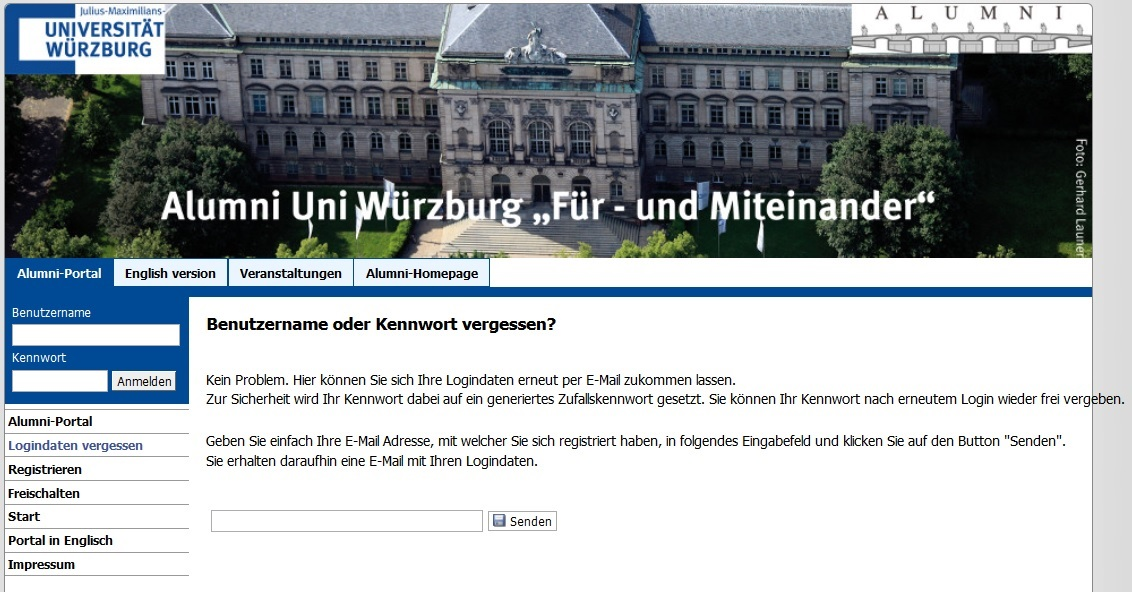
\includegraphics[width=\textwidth]{figures/Wiederherstellung_1.jpg}
		\caption{Wiederherstellungsformular für die Logindaten}
	\label{fig:Wiederherstellung_1}
\end{figure}

\subsubsection*{Positive Beobachtungen}
Der Bereich zum Wiederherstellen der Logindaten ist überschaubar gehalten. In zwei kurzen Textabschnitten wird dem Nutzer erklärt wie der Vorgang abläuft und was er dabei zu beachten hat. Das Formular besitzt nur ein einziges Eingabefeld und wirkt aufgeräumt. Der Nutzer hat nicht viel Spielraum für Fehlinterpretationen.

\problem{Text über den Rand hinaus geschrieben}{
Die Beschreibung zur Logindatenwiederherstellung wird über die Webseitenabgrenzung hinaus weiter geführt (siehe Abbildung \ref{fig:Wiederherstellung_1}). Die fehlende Formatierung des Textes wirkt unsauber und unprofessionell.
}{
Probleme solcher Art stören nicht direkt die Nutzung der Webseite, haben aber einen anderen negativen Effekt. Es stellt beim Nutzer die Seriosität des Portals in Frage, vor allem wenn an anderer Stelle nach vertraulichen Daten, beispielsweise der Bankverbindung, gefragt wird. Das ganze Auftreten des Alumni-Portals wird durch solche Formatierungsfehler in ein schlechtes Licht gerückt (Kategorie 1).
}{
Bei der Gestaltung von Texten sollte mehr Wert auf die Formatierung gelegt werden. Bestimmte Bereiche, in denen Text stehen kann, müssen auch zwingend eingehalten werden.
}\label{prob:rec:textueberrand}

\problem{Formularfeld nicht beschrieben}{
Das Formularfeld für die E-Mail-Adresse hat weder eine Beschreibung oberhalb, noch einen Platzhalter innerhalb des Feldes (siehe Abbildung \ref{fig:Wiederherstellung_1}). Es geht nur aus dem Text hervor welche Eingabe hier vom Nutzer verlangt wird.
}{
Die beiden beschreibenden Texte zur Wiederherstellung der Zugangsdaten erklären zwar den Nutzen des Inputfeldes, auf den ersten Blick wird dieser allerdings nicht ersichtlich. Warum im Vergleich zum Registrierungsformular an dieser Stelle die Beschreibung entfernt wurde, ist fraglich. Für den Nutzer ist somit auf den ersten Blick unklar ob hier eine E-Mail-Adresse, der Benutzername oder eine gänzlich andere Information verlangt wird (Kategorie 1).
}{
Das Formularfeld sollte um eine passende Beschreibung ergänzt werden, entweder mit einem Textfeld darüber oder als Platzhalter innerhalb.
}\label{prob:rec:formularnichtbeschrieben}

\problem{\emph{Senden} Button mit Diskettensymbol}{
Der Button zum Absenden des Wiederherstellungsformulars enthält ein Diskettensymbol (siehe Abbildung \ref{fig:Wiederherstellung_1}). 
}{
Üblicherweise wird das Diskettensymbol bei Programmen dazu genutzt die gerade bearbeiteten Daten, meist beim Nutzer selbst, zu speichern. In dem Kontext dieser Webseite steht das Symbol für das Speichern der vom Nutzer eingegebenen Daten in der Datenbank des Alumni-Portals. Die Symbolik könnte bei einem Nutzer, dem dieser Hintergrund nicht bekannt ist, für Verwirrung sorgen (Kategorie 1).
}{
Eine Beschriftung des Buttons, der die Funktion des Formulars knapp beschreibt, wäre hier angebracht. Beschriftungen, die beispielsweise \emph{Neu\-es Passwort anfordern} oder \emph{Neue Logindaten anfordern} lauten, wären sinnvoller.
}\label{prob:rec:sendenbutton}


\problem{Option für \glqq E-Mail-Adresse erkennen \grqq}{
Die Webseite bietet dem Nutzer den Service die Logindaten, also Benutzername und Passwort, zukommen zu lassen. Allerdings gibt es keine Option die zur Anmeldung verwendete E-Mail-Adresse erkennen zu lassen. Einige Webseiten bieten ihren Nutzern diesen Service an.
}{
Ein Ziel des Alumni Portals ist es mit Kommilitonen und Dozenten auch noch Jahre nach dem Abschluss in Kontakt bleiben zu können. Da sich in dieser Zeit durchaus die eigene E-Mail-Adresse ändern kann ist es sinnvoll einen solchen Service anzubieten.Per se handelt es sich hierbei allerdings nicht um ein Problem (Kategorie 0).
}{
Unter der Option \emph{Logindaten vergessen} befindet sich ein zu\-sätz\-li\-ches Formular, welches es dem Nutzer ermöglicht eine E-Mail-Adresse zu einem Benutzernamen erkennen zu lassen. Dabei wird eine E-Mail an die mit dem Benutzernamen verknüpfte Adresse versendet.
}\label{prob:rec:emailerkennen}

\begin{figure}
	\centering
		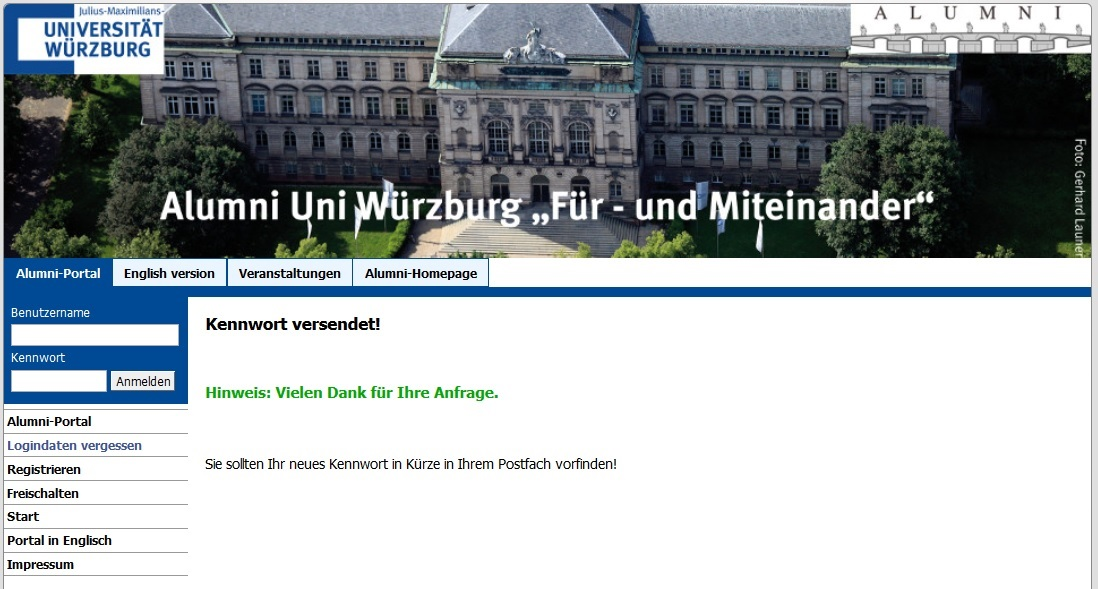
\includegraphics[width=\textwidth]{figures/Wiederherstellung_2.jpg}
		\caption{Feedback nach Absenden des Wiederherstellungsformulars}
	\label{fig:Wiederherstellung_2}
\end{figure}

\problem{Feedback-Meldung nicht konsistent mit anderen Meldungen}{
Nach dem Absenden des Formulars zur Wiederherstellung der Logindaten wird die gesamte Seite neu geladen. An Stelle des ausgefüllten Formulars erscheint eine fett gedruckte Benachrichtigung darüber, dass das Kennwort versendet wurde. Zusätzlich wird dem Nutzer mit einem grünen Text für seine Anfrage gedankt. In einer dritten Zeile wird in kleinerer Schriftgröße als in den anderen beiden Zeilen darauf hingewiesen, dass das neue Kennwort in Kürze im Postfach des Nutzers vorzufinden ist. In Abbildung \ref{fig:Wiederherstellung_2} sind diese drei unterschiedlichen Feedback-Nachrichten zu sehen.
}{
Feedback ist im Allgemeinen sehr wichtig für einen Nutzer, da er damit über den Status seiner Aktion mit dem System informiert werden kann. Im Fall der Passwortwiederherstellung erhält der Nutzer drei Nachrichten mit jeweils unterschiedlicher Darstellung des Textes. Darüber hinaus unterscheidet sich die Gestaltung anderer Feedback-Nachrichten derselben Webseite von Fall zu Fall. Das kann für Verwirrung beim Nutzer führen, da nicht ersichtlich ist, ob es einen Grund für die unterschiedlich gewählten Farben und Schriftgrößen gibt (Kategorie 1).
}{
Positives sowie negatives Feedback vom System sollte konsistent sein, das heißt es soll dieselbe Art und Weise einer Nutzerbenachrichtigung für die gesamte Webseite genutzt werden. Der Nutzer sollte unmissverständlich darüber in Kenntnis gesetzt werden, ob eine Interaktion mit der Webseite funktioniert hat und wenn nicht, worin der Fehler lag.
}\label{prob:rec:feedback1}

%#########################################################################
\usecasepart{Auslesen der Logindaten aus der E-Mail}
Das Formular wurde vom Nutzer ausgefüllt und abgesendet. Nun wartet dieser auf die E-Mail mit den neu generierten Logindaten. 

\subsubsection*{Positive Beobachtungen}
Die E-Mail mit neuen Logindaten wird sehr schnell zugestellt. In der Regel dauert es nicht länger als ein paar Minuten.

\problem{Formale Anrede in E-Mail fehlt}{
Wurde das \emph{Logindaten vergessen}-Formular ausgefüllt, so erhält der Nutzer eine E-Mail mit den neu generierten Zugangsdaten. Bei dieser E-Mail fällt sofort auf, dass die gesamte Anrede fehlt. Das Schreiben beginnt ohne jegliches Grußwort umgehend mit \emph{Ihre Zugangsdaten lauten wie folgt:} .
}{
Eine offizielle Webseite, wie in diesem Fall das Alumni-Portal, sollte mehr Wert auf die Umgangsform mit ihren Nutzern legen. Diese E-Mail verstärkt das Bild von mangelnder Professionalität und Seriosität und ist einzustufen in der Kategorie der schweren Probleme (Kategorie 3).
}{
Die E-Mail sollte, passend zum Nutzer, eine persönliche, formale Anrede enthalten.
}\label{prob:rec:anrede}

\problem{Fehlender Link zur direkten Anmeldung}{
In der E-Mail werden dem Nutzer die neu generierten Logindaten mitgeteilt. Ein Link, mit dem der Nutzer auf die Webseite geleitet, wird fehlt allerdings.
}{
Gewöhnlich befindet sich in einer E-Mail, mit der Userdaten oder Freischaltcodes versendet werde, ein Link, mit dessen Hilfe der Nutzer direkt auf die Webseite gelangt. Das verhindert einerseits den unnötigen Aufwand des Benutzers die Webseite manuell aufzurufen, andererseits können generierte Codes an den Link gehängt werden. Dabei würde gegebenenfalls das automatische Übertragen eines Freischaltcodes oder Passworts die Bedienung für den Nutzer erleichtern (Kategorie 2).
}{
Eine simple Verbesserung wäre ein Link mit dem ein Nutzer direkt zum Anmeldeformular kommt. Ebenfalls denkbar ist eine Umsetzung, bei der der Nutzer direkt auf ein Formular zur Passwortänderung geleitet wird. Dort wird er dann aufgefordert, ein neues Passwort zu setzen.
}\label{prob:rec:fehlenderlink}
%#########################################################################
\usecasepart{Anmelden mit neuen Logindaten}
Hat der Nutzer die E-Mail mit den neu generierten Logindaten erhalten, so ruft er die Webseite des Alumni-Portals auf, um sich damit das erste Mal einzuloggen. 

\subsubsection*{Positive Beobachtungen}
Das Anmelden mit den neuen Logindaten läuft ohne Probleme, es gibts nichts zu beanstanden.

%#########################################################################
\usecasepart{Setzen eines neuen Passworts}
Nach dem ersten Anmelden mit den neuen Logindaten wird ein Formular angezeigt, mit dem ein neues Kennwort gesetzt werden kann. 

\begin{figure}
	\centering
		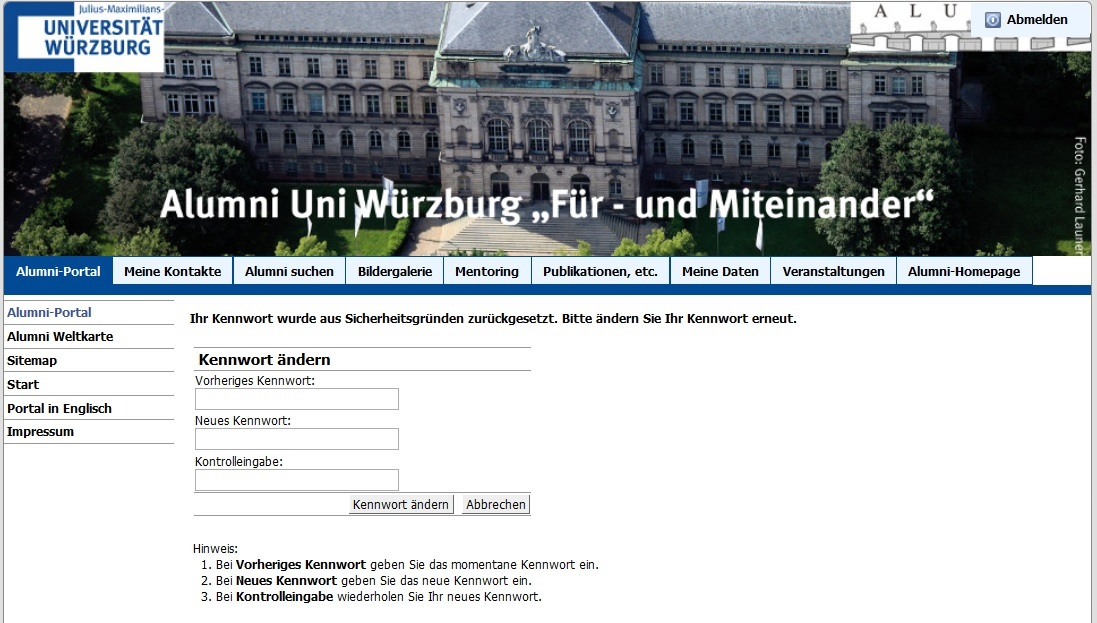
\includegraphics[width=\textwidth]{figures/Wiederherstellung_3.jpg}
		\caption{Formular zur Passwortänderung}
	\label{fig:Wiederherstellung_3}
\end{figure}

\subsubsection*{Positive Beobachtungen}
Die direkte Weiterleitung auf das Formular zum Ändern des Passwortes erleichtert dem Nutzer die Bedienung.

\problem{Fehlende Hinweise und Live-Validierung zu gültigen Passwörtern}{
Dem Formular zum Ändern des Passworts fehlt ein Hinweis darüber, welche Form ein Passwort haben muss oder darf. Es gibt weder einen Hinweis in Textform, noch gibt es irgendeine Art von Live-Validierung des Eingabefeldes (siehe Abbildung \ref{fig:Wiederherstellung_3}).}{
Ein Grund für das Wiederherstellen der Logindaten könnte darin bestehen, dass die Hinweise zu gültigen Kennwörtern bereits bei der Registrierung nicht ausreichend waren.\footnote{Beispiel: der fehlende Hinweis auf die Längenbegrenzung des Passworts auf 17 Zeichen.} Genau derselbe Fehler wird an dieser Stelle wiederholt. Bei dem Formular zur Änderung des Passworts steht kein Hinweis, wie eine gültige Passworteingabe auszusehen hat. Dieser Fakt ist äußerst ärgerlich für jeden Nutzer und mündet in Frustration. Ebenfalls wurde es versäumt eine Eingabevalidierung der Felder durchzuführen während das Passwort eingegeben wird bzw. wenn das Inputfeld verlassen wird. Lediglich beim Absenden des Formulars werden die Felder auf fehlerhafte Eingaben geprüft und der Nutzer darauf hingewiesen. Gerade bei Passwörtern ist das viel zu spät und damit nicht ausreichend. Störend und zugleich frustrierend ist dabei auch, dass die Eingabefelder nach dem erfolglosen Absenden geleert werden (Kategorie 4).
}{
Abhilfe schafft ein einheitlicher Hinweistext, wann ein Passwort vom System akzeptiert wird und wann nicht. Ein solcher Hinweis könnte bei Eingaben des Nutzers leicht hervorgehoben werden, sobald dieser in das jeweilige Formularfeld klickt. Damit würde der Nutzer bei der Passwortwahl direkt darauf aufmerksam gemacht werden. Die fehlende Eingabevalidierung sollte ebenfalls implementiert werden. Durch direktes Feedback kann der Nutzer umgehend erkennen, was er bei der Passwortwahl beachten muss oder vielleicht vergessen hat.
}\label{prob:rec:validierung}

\problem{Feedback bei der Passwortänderung}{
Das Feedback bei der Passwortänderung erscheint zwischen der oberen Navigationsleiste und dem Formular zur Passwortänderung. Der Einzeiler zur erfolgreichen Kennwortänderung entspricht wiederum nicht den anderen Feedbackmeldungen.
}{
Wie bereits bei den anderen Feedbackmeldungen bemängelt zeigt sich auch hier wieder eine Inkonsistenz zum Rest der Webseite (Kategorie 1).
}{
Ein mögliches Feedback sollte auch an dieser Stelle den Nutzer über die erfolgreiche Passwortänderung informieren. Eine solche Meldung sollte konsistent mit allen anderen Meldungen des Systems an den Nutzer sein. 
}\label{prob:rec:feedback2}

\subsubsection*{Fazit: Wiederherstellung der Logindaten}
Die Wiederherstellung der Logindaten ist funktionell, bietet aber noch deutliches Verbesserungspotenzial. In der bisherigen Version wird der Nutzer in der korrekten Bedienung behindert (z.B. durch fehlende Hinweise zur Auswahl von gültigen Passwörtern). Durch kleine Verbesserungen kann der Bedienungskomfort für den Nutzer gesteigert werden.














%Thomas
\newpage
\usecase{Besucher sucht einen ehemaligen Kommilitonen}
\usecasepart{Anmeldung am Alumni-Portal}

\subsubsection*{Positive Beobachtungen}
Das Anmeldeformular für das Portal ist an einer zentralen und gut einsehbaren Stelle positioniert. Dadurch ist es direkt im Blickfeld des Nutzer und kann jederzeit seine Verwendung finden. Zwei Eingabefelder ermöglichen das Eintippen der Zugangsdaten, mit denen sich der Benutzer am Portal authentifizieren kann. Unklarheiten bezüglich der einzugebenden Daten entstehen durch die klare Struktur und die Beschriftung der Elemente nicht. Der Button \emph{Anmelden} führt wie erwartet den Login aus. Abschließend ist positiv anzumerken, dass nach Absenden des Formulars der Benutzer visuelles Feedback eingeblendet bekommt. Dadurch wird veranschaulicht, dass das System die Anfrage zum Login bearbeitet.

\problem{Dezentes Feedback bei fehlerhaftem Login}
{
	Erfolgt eine fehlerhafte Eingabe von Benutzername und Passwort durch\-läuft das System den kompletten Vorgang der Anmeldung. Die Login-Daten werden verarbeitet und abschließend wird die Portalseite neu geladen. Befindet sich der Nutzer zum Zeitpunkt des Login nicht auf der Startseite, so wird er dorthin weitergeleitet. Die neu aufgebaute Startseite blendet dem Nutzer Feedback in Form eines kurzen Hinweistextes ein. Dieser teilt mit, dass aufgrund ungültiger Zugangsdaten die Authentifizierung nicht möglich war. Die Platzierung sowie Formatierung des Feedback ist sehr schlicht und unauffällig gewählt. Unerfahrene Anwender übersehen eine derartige Fehlermeldung unter Umständen und warten auf eine Reaktion von Seiten des Systems.
}
{
	Das aufgeführte Problem ist nicht derart schwerwiegend, als dass es die Funktionalität der Seite in irgendeiner Form einschränkt. Durch verminderte Aufmerksamkeit des Anwenders kann es jedoch dazu führen, dass wichtiges Feedback schlichtweg nicht wahrgenommen wird. Somit ist die Art und Weise der Rückmeldung von Webseite an Benutzer nicht auffällig genug gestaltet. Aus den genannten Gründen lassen sich diese Umstände der Kategorie als \emph{mittelschweres Problem} zuordnen (Kategorie 2).		
}
{
	Ziel ist es, dass der Nutzer eingeblendetes Feedback, welches vom System erzeugt wird, auffällig und gut sichtbar präsentiert bekommt. Deshalb empfiehlt sich eine entsprechende Farbgestaltung: rot für Fehlermeldungen, gelb für Warnungen und grün für erfolgreich durchgeführte Aktionen. Weiterhin ist die Schriftgröße angemessen zu wählen. Eine einheitliche Platzierung des Feedback ist ebenso erstrebenswert. Bei Eingabefeldern ist es beispielsweise empfehlenswert fehlerhafte Eingaben und dazugehörige Hinweistexte in unmittelbarer Nähe des betroffenen Elements zu platzieren.
}
\label{prob:suche:loginfehler}


% Aufgabenteil
% ------------
\usecasepart{Aufrufen der Suchmaske über das Menü}

\subsubsection*{Positive Beobachtungen}
Das horizontal angelegte Menü unterhalb der Headergrafik ist schlicht und übersichtlich gehalten. Die darin aufgelisteten Menüpunkte sind eindeutig und leicht verständlich beschrieben. Weiterhin lässt deren Benennung einen direkten Rückschluss darauf zu, welche Funktionalität der Benutzer dahinter zu erwarten hat. So ist beispielsweise direkt ersichtlich, dass sich hinter dem Punkt \emph{Alumni suchen} im Menü eine Suchmaske befindet.

\problem{Suchanfrage startet unverzüglich nach Seitenaufbau}
{
	Nach einem Klick auf \emph{Alumni suchen} im Menü öffnet sich direkt die Suchmaske zur Eingabe von Kontaktdaten. Zu diesem Zeitpunkt ist das Suchfeld vom Anwender unberührt: es erfolgte bisher keine Eingabe. Nach dem erfolgreichen Seitenaufbau startet unaufgefordert der Suchvorgang mit einem leeren Suchbegriff. Als Ergebnis vermeldet das System, dass keine passenden Datensätze zu der Suche vorhanden sind. Dem Benutzer werden zusätzlich Elemente zur Navigation (vorwärts und rückwärts blättern) innerhalb der Trefferliste angezeigt. Das Ausführen der Funktionalität der beschriebenen Navigationselemente ist bei leerem Ergebnis nicht möglich.
}
{
	Das sofortige starten eines Suchvorgang trotz fehlender Eingabe wirkt deplatziert und ist überflüssig. Die eingeblendeten Elemente für das Blättern in der Ergebnisliste bieten dem Anwender ebenfalls kein Mehrwert. Bedienung und Funktionalität der Webseite sind aufgrund des beschriebenen Sachverhaltes nicht eingeschränkt. Hierbei handelt es sich um ein \emph{mittelschweres Problem} (Kategorie 2).
}
{
	Das Auslösen der Suche nach dem vollständigen Aufbau der Seite entfernen. Dadurch lässt sich sowohl die Ladezeit des Inhaltes, als auch eine überflüssige Abfrage an die Datenbank einsparen. Weiterhin sollten dem Nutzer keine überflüssigen Funktionselemente angezeigt werden, für die er zum derzeitigen Zeitpunkt keine Verwendung findet.
}
\label{prob:suche:suchanfrage}

% Aufgabenteil
% ------------
\usecasepart{Auswahl der gewünschten Suchmaske}
%\subsubsection*{Positive Beobachtungen}
%... 

\problem{Seitenmenü unübersichtlich/inkonsistent gestaltet}
{
	Im linken Bereich auf der Unterseite \emph{Alumni suchen} befindet sich ein zusätzliches Menü, über welches der Nutzer die Eingabemaske für die Suche wechseln kann. Zur Veranschaulichung dient die Abbildung \ref{fig:suche:seitlichesmenue}. Die Visualisierung der vertikal angelegten Menüelemente (Farbe und Formatierung) ist unüblich gewählt. Es ist nicht eindeutig erkennbar, welcher Menüpunkt als aktiv gesetzt ist. Dem Anwender fehlt somit das Verständnis, welche Suchmaske ihm aktuell angezeigt wird. Bekannte Mouse-Over Effekte bei Hyperlink-Elementen finden in der Menüleiste keine Verwendung. Die dort eingesetzte Farbe Schwarz in einem Navigationselement ist ebenfalls von Nachteil. Für gewöhnlich gehen Nutzer bei dieser Formatierung von normalen Textelementen aus und erwarten nicht einen Link zum Klicken.
	\begin{figure}[h]
		\centering
		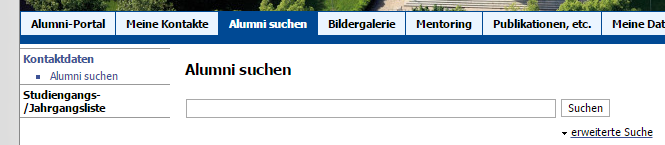
\includegraphics[scale=0.75]{figures/seitliches_menue.png}
		\caption{Seitenmenü bei der Suche nach einem Alumni}
		\label{fig:suche:seitlichesmenue}
	\end{figure}
}
{
	Die ungewöhnliche Wahl der Formatierung für Hyperlinks und die fehlende Hervorhebung des aktiv gewählten Menüelements sorgt beim Endanwender für Verwirrung. Dies wiederum führt zur falschen Verwendung der im Menü angebotenen Aktionen. Aufgrund dieser Umstände lässt sich das Problem in die Kategorie \emph{mittelschweres Problem} einstufen. Die Funktionalität der Webseite ist hierdurch nicht eingeschränkt (Kategorie 2).
}
{
	Das seitliche Menü im unmittelbaren Blickfeld des Anwender platzieren. Hierfür bietet sich die Positionierung als zusätzliche horizontale Navigation im Inhaltsbereich der Suchseite an. Dadurch wird die Aufmerksamkeit des Nutzers angezogen und die Existenz der unterschiedlichen Eingabemasken hervorgehoben. Zudem empfiehlt sich die Formatierung von Hyperlink-Elementen an die Gewohnheiten erfahrener Nutzer anzupassen: unterstreichen, eine eigene Farbe für Links und einen angemessenen Mouse-Over Effekt dieser Elemente.
}
\label{prob:suche:seitenmenue}

% Aufgabenteilgit p
% ------------
\usecasepart{Alumni über einen Suchbegriff finden}
%\subsubsection*{Positive Beobachtungen}
%... 

\problem{Suchvorgang mit fehlender Eingabe ausführbar}
{
	Eine Eingabe in die Suchmaske ist nicht zwingend erforderlich. Dem Anwender wird gestattet einen Suchvorgang mit leerer Eingabe zu starten. Nach einem Neuaufbau der Seite wird ein visuelles Feedback eingeblendet, das darauf hinweist, dass mindestens ein Suchbegriff notwendig ist. Trotz gescheiterter Suche wird wiederum eine leere, nicht benötigte Trefferliste mit dazugehörigen Elementen zur Navigation angezeigt.
}
{
	Das beschriebene Probleme schränkt den Anwender der Webseite hinsichtlich Bedienung und Funktionalität nicht ein. Die Tatsache, dass eine leere Suche nicht im Vorfeld bereits von Seiten des System unterbunden wird, kann beim Benutzer jedoch auf Unverständnis treffen. Insgesamt lässt sich dieser Umstand als \emph{mittelschweres Problem} einstufen (Kategorie 2).
}
{
	Eine denkbare Lösung ist es, den Button zum Starten der Suche so lange zu deaktivieren, bis der Endanwender mindestens ein Suchbegriff/-wort eingegeben hat. Danach kann der Suchvorgang wie gewohnt über den danebenliegenden Button gestartet werden. Ein alternativer Verbesserungsvorschlag ist es, dem Nutzer unmittelbar Feedback zu präsentieren und ihn auf das Fehlen eines Suchbegriffs hinzuweisen. Dadurch wird ein unnötiges Neuladen der Webseite verhindert, sowie die damit verbundenen Wartezeit während die Seite sich aktualisiert.
}
\label{prob:suche:leereeingabe}

\problem{Keine eindeutige Festlegung für Eingabe in das Suchfeld}
{
	Bei der Suche nach einem Alumni anhand von Kontaktdaten ist die Eingabe in das vorgesehene Feld nicht eindeutig festgelegt. Intuitiv geht der Nutzer davon aus, dass er den Namen der zu suchenden Person in das Eingabefeld eingeben soll. Bei einem ausführlichen Test wird ersichtlich, dass alle personenbezogenen Daten Gegenstand einer Suchenanfrage sein können. Darunter fällt beispielhaft der Wohnort, der Straßenname, die E-Mail Adresse, sowie derzeitige Tätigkeit und Firma in der die Person arbeitet.
}
{
	Die Suche funktioniert auf den ersten Blick so wie es der Nutzer erwartet. Ein Suchbegriff wird eingegeben und daraufhin werden alle Ergebnisse eingeblendet, die eben diesen String  beinhalten. Da nicht kommuniziert wird, welche Eingabe vom Anwender erwartet wird, ist nicht eindeutig vorhersehbar, mit welchen persönlichen Daten der Alumni die Sucheingabe abgeglichen wird. Der Umstand einer fehlenden Information hinsichtlich zu tätigender Eingabe lässt dieses Problem der Katgorie \emph{mittelschweres Problem} zuordnen (Kategorie 2).
}
{
	Da die Webseite dem Benutzer eine erweiterte Suchfunktionalität anbietet, ist es denkbar die grundlegende Sucheingabe auf den Vor- und Nachnamen der zu suchenden Person zu beschränken. Ein erklärender Hinweis für den Benutzer hinsichtlich gültiger Eingabewerte ist notwendig. Eine Suche mit spezifischen Angaben zur Person sollte künftig über die erweiterten Suchoptionen getätigt werden.
}
\label{prob:suche:eingabeuneindeutig}

\problem{Anzeige der Trefferanzahl während Sucheingabe}
{
	Tippt der Nutzer einen Suchbegriff ein, so wird umgehend eine Abfrage an die Datenbank gesendet, welche die Anzahl an Treffern zu dieser Eingabe zurückliefert. Erkenntlich ist dies an der Lade-Animation rechts neben dem Eingabefeld, wo nach erfolgreicher Abfrage das Resultat angezeigt wird. Diese Funktionalität bietet dem Anwender zum genannten Zeitpunkt der Eingabe keinerlei wertvollen Informationsgehalt. Zumal der Suchvorgang explizit über den Button \emph{Suchen} gestartet werden muss bevor eine Trefferliste angezeigt wird. Das eingeblendete Ladesymbol kann den Endanwender zusätzlich verwirren, der die Eingabe unter Umständen noch nicht beendet hat. Das System vermittelt jedoch den Eindruck, als würde die Suchabfrage bereits durchgeführt werden.}
{
	Das unmittelbar während der Eingabe erscheinende Ladesymbol und die noch nicht abgeschickte Suche können den Nutzer aus dem Konzept bringen. Zudem ist die Position, sowie die Art des Feedbacks zum Zeitpunkt der Eingabe für den Nutzer in dieser Art und Weise wertlos. Hierbei handelt es sich bereits um ein \emph{schweres Problem} (Kategorie 3).
}
{
	Zum Zeitpunkt der Eingabe kann der Nutzer sehr gut auf die Anzahl der Treffer mit dem eben eingetippten Suchbegriff verzichten. Aus diesem Grund sollte die zudem wenig aussagekräftige Information vollständig weggelassen werden. Durchaus interessanter --- und vom Informationsgehalt wertvoller --- dürfte eine Autovervollständigung sein. Diese schlägt dem Nutzer während der Eingabe mögliche Vervollständigungen vor, die aufgrund des bereits eingegebenen String und dem Datenbestand der Alumni Benutzerliste getroffen werden können.
} 
\label{prob:suche:trefferanzeige}

\problem{Suchvorgang durchsucht alle Datenfelder}
{
	Im vorherigen Verlauf des Walkthrough ist das Problem beschrieben, dass die Sucheingabe nicht eindeutig festgelegt ist. Betrachten wir im Anschluss nun die Ergebnisliste einer Suche genauer. Es fällt auf, dass Treffer aufgelistet sind, die aufgrund der Eingabe für den Suchenden nicht relevant sind. Bei dem Betrachten der Profilseite der nicht relevanten Treffer wird ersichtlich, dass alle Angaben zur Person mit dem eingegebenen Begriff abgeglichen werden. So findet das Portal bei dem Suchstring \glqq .de\grqq ~alle Nutzer, die sich mit einer .de E-Mail-Adresse angemeldet haben. Ein weiteres Beispiel: die Anschrift eines Alumni beinhaltet einen Vornamen (z.B. Anna-Straße 24).
}
{
	Aus Sicht des Nutzers arbeitet die Suchfunktion nicht nach den eigenen Vorstellungen und führt die Aktion fehlerhaft aus. Intuitiv geht der Endanwender davon aus, dass mit der normalen Suchfunktion vorrangig nach dem Namen eines Alumni gesucht werden kann. Tauchen in der Trefferliste Personen auf, deren Namen komplett von der Eingabe abweichen, so stößt dies auf Unverständnis und verwirrt den Nutzer. Bei dieser fehlerhaften und unerwarteten Funktionalität handelt es sich um ein \emph{fa\-ta\-les Problem} (Kategorie 4).
}
{
	Bei der Sucheingabe muss festgelegt sein, welche Eingaben dem Nutzer gestattet sind und dadurch ersichtlich werden, welche Ergebnisse zu erwarten sind. Im vorliegenden Szenario ist es sinnvoll die normale Suche lediglich auf den Namen zu beschränken und dies im Eingabefeld per \glqq Hint\grqq ~vorzugeben. Für eine detaillierte Suche steht dem Suchenden zudem ein entsprechendes Formular mit erweiterten Eingabemöglichkeiten zur Verfügung. Mit Hilfe von diesem ist es ihm gestattet seine Suche weiter zu verfeinern.
} 
\label{prob:suche:sucheallefelder}

% Aufgabenteil
% ------------
\usecasepart{Alumni über erweiterte Suchoptionen finden}

\subsubsection*{Positive Beobachtungen}
Das ausgeklappte, erweiterte Suchmenü wirkt auf den Benutzer ordentlich gegliedert und auf den ersten Blick aufgeräumt. Die zu tätigenden Eingaben sind nach Obergruppen (private und geschäftl. Kontaktdaten) strukturiert und beinhalten die zugehörigen Eingabefelder.

\problem{Zu viele Eingabefelder für den Nutzer}
{
	Die Eingabefelder sind gruppiert und wirken auf den ersten Blick aufgeräumt. Bei näherem Betrachten fällt jedoch der hohe Detailgrad auf, mit dem die Suche ausgefüllt werden kann. Viele der anzugebenden Informationen stehen dem Suchenden im Regelfall nicht zur Verfügung und sind unbekannt. Durch diese Umstände wirkt die Eingabemaske unnötig überladen.
}
{
	Die Funktionalität der Webseite sowie die Suchfunktion sind aufgrund der Fülle an Eingabemöglichkeiten in keinster Weise eingeschränkt. Eine derart umfangreiche Suchmaske schreckt den Benutzer oftmals vor dem Ausfüllen ab. Es handelt sich um ein \emph{leichtes Problem} (Kategorie 1).
}
{
	Um dem Benutzer eine komfortable und schnelle Eingabe erweiterter Suchoptionen zu ermöglichen, bietet es sich an diese stark zu reduzieren. Dazu können überflüssige, bzw. zu detaillierte Formularfelder, bezüglich Werdegang und geschäftlichen Kontaktdaten, herausgenommen werden. Es macht wenig Sinn anhand zu spezifischer Kriterien eine Suche nach ehemaligen Kommilitonen/Alumni-Mitgliedern zu starten.
}
\label{prob:suche:vieleeingabefelder}

\problem{Speichern/Laden der Suche nicht implementiert}
{
	Dem Anwender wird am Fuß der erweiterten Suchmaske die Funktionalität angeboten, das ausgefüllte Formular zu speichern und bei späteren Suchanfragen wieder zu verwenden. Das Gegenstück hierzu --- eine zuvor ausgefüllte Suche laden --- ist ebenfalls über einen Hyperlink erreichbar. Nach Klick auf \emph{Suche speichern} wird der Anwender aufgefordert eine Bezeichnung für die ausgefüllte Suche zu vergeben (siehe Abb. \ref{fig:suche:speichern}). Hinter dem Button \emph{Speichern}, um die Eingabe zu persistieren, verbirgt sich jedoch keine Funktionalität. Das Abspeichern der Suchmaske ist beim derzeitigen Stand der Webseite nicht implementiert. Umgekehrt ist das Laden einer zuvor gespeicherten Suche nicht durchführbar, da die Funktionalität \emph{Suche speichern} nicht verwendbar ist.
	\begin{figure}[h]
		\centering
		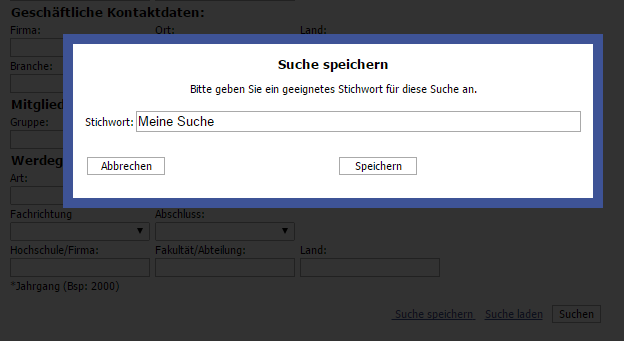
\includegraphics[scale=0.75]{figures/suche_speichern.png}
		\caption{Dialog für das Speichern einer Suchmaske}
		\label{fig:suche:speichern}
	\end{figure}
}
{
	Bei der beschriebenen Situation handelt es sich um einen klaren \glqq Showstopper\grqq . Dem Benutzer wird eine Funktionalität zur Verfügung gestellt, die allerdings nicht die erwartete Aktion ausführt. Sie bewirkt keinerlei Aktion. Aus diesem Grund handelt es sich um ein \emph{fatales Problem}, das den Anwender hinsichtlich angebotener Funktionalität der Webseite einschränkt (Kategorie 4).
}
{
	Eine Möglichkeit besteht darin, das Abspeichern der Suchmaske zu implementieren. Dadurch erhält der Benutzer die zuvor beschriebene Funktionalität geboten und kann diese wie erwartet einsetzen. Alternativ kann die Funktion \emph{Suche speichern} komplett von der Webseite entfernt werden. Es ist eher ungewöhnlich das Speichern einer Suchmaske anzubieten. Ein sinnvoller Anwendungsfall tritt nur selten auf und die Funktionalität bietet geringen Mehrwert für den Nutzer des Systems.
}
\label{prob:suche:suchespeichern}

% Aufgabenteil
% ------------
\usecasepart{Alumni über die Studiengangliste finden}

\subsubsection*{Positive Beobachtungen}
Durch die große Anzahl verschiedener Studiengänge wird die daraus resultierende Liste sehr lang. Mit Hilfe der bereitgestellten Filter wird dem Anwender ein hilfreiches Werkzeug an die Hand gegeben, um den Umfang der Auflistung stark zu reduzieren. Dies ist ihm sowohl anhand des Anfangsbuchstaben gestattet, als auch in Form einer Jahreszahl für Beginn sowie Ende der Studienzeit. 

\problem{Fehlendes Feedback beim Laden der Studiengangsliste}
{
	Entscheidet sich der Nutzer einen Alumni anhand des Studiengangs zu suchen, so nutzt er die Suchfunktion hinter dem Menüpunkt \emph{Studiengangs-/Jahrgangsliste} in der linken Navigation. Nach dem Klick präsentiert sich dem Anwender zunächst ein leerer Inhaltsbereich. Zu diesem Zeitpunkt meldet das System kein Feedback an den Nutzer. Es ist in dieser Situation nicht ersichtlich, ob der Ladevorgang abgeschlossen, abgebrochen oder noch in Arbeit ist. Der Benutzer erhält den Eindruck als befände er sich auf einer Unterseite ohne entsprechenden Inhalt. Erst nach längerer Wartezeit erscheint die Liste aller Studiengänge.
}
{
	Das System berichtet dem Anwender nicht den aktuellen Zustand der Aktion. Es ist nicht ersichtlich, ob in absehbarer Zeit die Aktion beendet und der erwartete Inhalt angezeigt wird. Die beschriebene Thematik lässt sich als \emph{fatales Problem} einstufen (Kategorie 4). Aufgrund des fehlenden Feedbacks vom System wird der Nutzer die Unterseite höchst wahrscheinlich vorzeitig verlassen. 
}
{
	Abhilfe schafft das Anzeigen von Feedback für den Nutzer. Die einfachste Möglichkeit hierfür ist eine Animation in Form eines Ladebalken oder “Spinner”, die dem wartenden Benutzer angezeigt wird. Dadurch wird signalisiert, dass das System im Hintergrund noch arbeitet und in absehbarer Zeit das Ergebnis präsentiert wird.
}
\label{prob:suche:keinfeedback}

\problem{Unübersichtliche Darstellung der Studiengangsliste}
{
	Die Liste, welche alle eingetragenen Studiengänge beinhaltet, erstreckt sich über eine Spalte und kann entsprechend sehr lang werden. Durch die relativ kurzen Bezeichnungen der Studiengänge wird die Breite des Inhaltsbereichs nicht vollständig ausgeschöpft. Es wird vom Nutzer erwartet, dass er entsprechend weit auf der Webseite nach unten scrollt. Nur so ist es ihm gestattet, alle Einträge der Liste sehen zu können.
}
{
	Bei dieser Problembeschreibung handelt es sich lediglich um geringe Mängel am User-Interface. Es sind dadurch keinerlei Einschränkungen der Funktionalität gegeben. Die Umstände lassen sich als \emph{leichtes Problem} einordnen (Kategorie 1).
}
{
	An dieser Stelle bietet sich ein mehrspaltiges Layout für die Liste aller Studiengänge an. Hiermit wird der Inhaltsbereich besser ausgenutzt und es entsteht beim Anwender nicht der Eindruck einer unendlichen Auflistung. Die Studiengänge lassen sich somit viel schneller auffassen ohne auf der Webseite weit nach unten scrollen zu müssen.
}
\label{prob:suche:studiengangsliste}

\problem{Ungültige Studiengänge erscheinen in der Liste}
{
	In der Studiengangliste sind zum Teil fehlerhafte und mit Rechtschreibfehlern behaftete Studiengänge aufgelistet. Diese entstehen unter anderem bei der Registrierung durch einen neuen Benutzer am Alumni-Portal. Das Anmeldeformular gestattet bei der Registrierung die Eingabe von individuellen Studiengängen, wodurch fehlerhafte Eingaben entstehen können.
}
{
	Aufgrund des falsch zugeordneten Studiengangs im Profil eines Alumni ist es durchaus möglich, dass der Benutzer das gewünschte Mitglied nicht finden kann. Somit ist das Ziel dieses Use-Case theoretisch nicht erreichbar. Es handelt sich um ein \emph{schweres Problem} (Kategorie 3).
}
{
	Derartige Fehleingaben bei der Registrierung lassen sich durch eine Validierung der Eingabedaten des entsprechenden Formulars verhindern. Dieser Lösungsvorschlag ist jedoch nicht Bestandteil von diesem Use-Case, sondern wird in Kapitel \ref{usecse:reg} (\nameref{usecse:reg}) ausführlich behandelt.
}
\label{prob:suche:ungueltigestudiengaenge}

% Aufgabenteil
% ------------
\usecasepart{Sichten der Trefferliste einer Suche}

\subsubsection*{Positive Beobachtungen}
Die Trefferliste ist übersichtlich und gut strukturiert aufgebaut. Die einzelnen Resultate heben sich mit Hilfe unterschiedlicher Hintergrundfarben gut voneinander ab. Zudem erhält der Endanwender direkt in der Ergebnisliste die ersten wichtigen Informationen zu den Personen, wie der aktuelle Wohnort, ein Profilbild (sofern vorhanden) und den vollständigen Namen. Weiterhin positiv anzumerken sind die Blätter-Elemente mit deren Hilfe der Anwender durch die gesamte Ergebnisliste navigieren kann. Dabei stehen ihm folgende Funktionen zur Verfügung: vorwärts und rückwärts blättern, sowie an den Anfang bzw. das Ende der Trefferliste springen. 

\problem{Hinweis \glqq Unbekannter Typ\grqq ~bei Suchtreffern}
{
	In der Liste aller Treffer erscheint bei einzelnen Resultaten der Hinweistext \glqq Unbekannter Typ\grqq ~in rot und fett gedruckter Schrift (siehe Abb. \ref{fig:suche:unbekanntertyp}). Dieser ist zurück zu führen auf eine  fehlende Eingabe im persönlichen Profil des betroffenen Alumni. Dieser Hinweistext hat für den Anwender keinerlei Informationsgehalt und trägt viel mehr zur Verwirrung bei. Der Grund für diesen auffällig gestalteten Text ist für den Suchenden nicht ersichtlich. Die Aufmerksamkeit des Nutzers wird unnötigerweise auf diesen Hinweis gezogen.
	\begin{figure}[h]
		\centering
		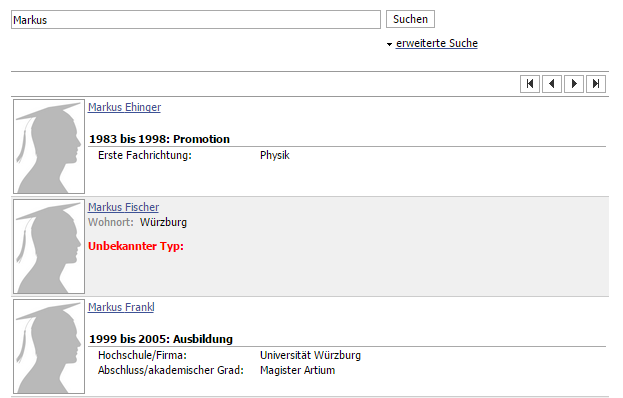
\includegraphics[scale=0.75]{figures/unbekannter_typ.png}
		\caption{Ergebnisliste mit Treffer \glqq Unbekannter Typ\grqq}
		\label{fig:suche:unbekanntertyp}
	\end{figure}
}
{
	 Die eingeblendete Profilinformation ist für den Benutzer nicht nachvollziehbar, schränkt die Funktionalität der Webseite allerdings nicht ein. Aus diesem Grund ist diese Auffälligkeit lediglich der Kategorie \emph{mittelschweres Problem} zuzuordnen (Kategorie 2).
}
{
	Handelt es sich um eine fehlende Eingabe von Seiten des entsprechenden Alumni kann dieser Hinweistext ebenso gut ausgeblendet und nicht präsent sein. Dadurch stellt sich dem Suchenden nicht die Frage, welche Informationen damit verbunden sind. Eine alternative Verbesserung ist es die Meldung mit mehr Informationsgehalt auszustatten, so dass der Benutzer versteht, wieso an dieser Stelle ein auffälliger Hinweistext angezeigt wird.
}
\label{prob:suche:unbekanntertyp}

\problem{Trefferanzahl pro Seite und Blätterfunktion}
{
	Bei den Suchergebnissen ist die Anzahl der Treffer fest auf fünf pro Seite festgelegt. Dadurch ist der Anwender gezwungen sehr oft zu blättern, sofern sich der gesuchte Alumni mindestens in der zweiten Hälfte der Liste befindet. Dabei wird auch die eingeschränkte Funktionalität ersichtlich, zwischen den Seiten der Ergebnisliste hin und her zu springen. Es ist dem Anwender nur gestattet eine Seite vor- bzw rückwärts zu blättern, bzw. direkt an den Anfang/das Ende der Trefferliste zu springen. Die Bedienung der Blätterfunktion ist somit aus Sicht des Nutzers stark eingeschränkt und gestaltet die Bedienung ineffizient und unangenehm.
}
{
	Die Funktionalität und Handhabung der Webseite ist durch dieses Problem nicht vollständig eingeschränkt. Durch die festen Vorgaben von Seiten des System (Anzahl Treffer pro Seite, nur eine Seite vor- oder zurückblättern) werden dem Nutzer diesbezüglich keinerlei Freiheiten eingeräumt. Die beschriebene Problematik lässt sich der Kategorie \emph{mittelschweres Problem} zuordnen (Kategorie 2).
}
{
	Die Anzahl der Treffer pro Seite lassen sich variabel gestalten. Der Nutzer kann per Drop-Down Menü selbst bestimmen wie viele Resultate auf einer Seite angezeigt werden sollen. Die Blätterfunktion lässt sich dahingehend verbessern, dass nicht nur ein Vorwärts- und Rückwärts-Button angeboten wird. Das Element zum Navigieren wird hierzu komplett umgestaltet. Wie diese Navigation aussehen kann, verdeutlicht Abb. \ref{fig:suche:pagination}.
	
	\begin{figure}[h]
		\centering
		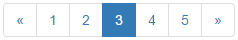
\includegraphics[scale=0.75]{figures/pagination.png}
		\caption{Navigationselemente für Ergebnisliste einer Suche}
		\label{fig:suche:pagination}
	\end{figure}
}
\label{prob:suche:trefferanzahl}

\subsubsection*{Fazit: Nutzersuche}
Abschließend lässt sich sagen, dass sich die Suchfunktion auf dem Alumni-Portal als nützlich und funktionell erwiesen hat. Dem Nutzer ist somit gestattet sein Ziel zu erreichen: einen ehemaligen Kommilitonen zu finden. Bei der durchgeführten Evaluation sind einige Probleme aufgetaucht, die die Verwendung der Suche zum Teil erheblich erschweren und für den Nutzer unangenehm erscheinen lassen. Dazu zählen mangelndes Feedback auf ausgeführte Aktionen, bis hin zu nicht implementierten Funktionen. Durch eine Verbesserung der Kommunikation vom System zum Anwender lassen sich viele der zuvor aufgeführten Probleme lösen. Die als fatal und schwerwiegend kategorisierten Probleme sollten in einer überarbeiteten Version der Webseite definitiv behoben werden.


\section{Fazit}\label{sec:fazit}
Für die Evaluation wurde ein typischer Use-Case gewählt. Er beinhaltet das Besuchen der Startseite, gefolgt von einer Registrierung inklusive Freischaltung und/oder Zurücksetzen des Passworts sowie die Suche nach ehemaligen Kommilitonen. 
Im Rahmen dieses Use-Case haben sich bereits schwerwiegende Probleme hinsichtlich User-Interface und Kommunikation in Form von Feedback mit dem Nutzer gezeigt. Das Portal bleibt dabei in mehreren Aspekten hinter dem aktuellen Standard moderner Webseiten zurück. 

Zusammenfassend lässt sich sagen, dass die Webseite des Alumni-Portals deutliche Schwächen aufweist. Dissonanzen zwischen den Erwartungen des Nutzers und der Reaktion der Webseite sind ein häufiges Problem.
Zurückführen lässt sich dies überwiegend auf die mangelnde Kommunikation von Informationen und Systemfeedback an den Nutzer.
Zum Teil werden gar Funktionen beworben, die schlichtweg nicht Bestandteil der aktuellen Implementierung der Webseite sind.

Abschließend hinterlässt das Alumni-Portal der Universität Würzburg aufgrund der aufzeigten Mängel einen unprofessionellen und unseriösen Eindruck. 
Da das Portal die Universität und den Alumni-Verein repräsentiert, hat ein qualitativ schlechter Internetauftritt auch einen negativen Einfluss auf die Außenwirkung und den Ruf der Universität Würzburg. 


%bisher nur die bib aus dem example report
%\bibliography{report}

\newpage
\appendix

\section{Designalternativen}
BLABLA, weitere Sachen die uns aufgefallen sind, die aber nicht Bestandteil unseres Walkthroughs waren
\section{Auflistung der Probleme sortiert nach Schwere}

\subsection*{Kategorie 4: Fatales Problem}
\begin{tabular}{|p{12cm}|c|}
\hline
\textbf{Beschreibung} & \textbf{Abschnitt} \\
\hline\hline
\nameref{prob:start:weltkarte} & \ref{prob:start:weltkarte} \\ 
\nameref{prob:start:popup} & \ref{prob:start:popup}\\
\nameref{prob:start:seitenmenue} & \ref{prob:start:seitenmenue}\\
Grüner Fehlertext bei der Passwortwahl & \ref{prob:frei:warntextgruen}\\
Längenbeschränkung des Passwortfeldes & \ref{prob:frei:passwortlaenge}\\
\hline
\end{tabular}

\subsection*{Kategorie 3: Schweres Problem}
\begin{tabular}{|p{12cm}|c|}
\hline
\textbf{Beschreibung} & \textbf{Abschnitt} \\
\hline\hline
\nameref{prob:start:panel} & \ref{prob:start:panel} \\
\nameref{prob:start:pkt:reg} & \ref{prob:start:pkt:reg}\\
\nameref{prob:start:pkt:frei} & \ref{prob:start:pkt:frei}\\
\nameref{prob:start:pkt:start} & \ref{prob:start:pkt:start}\\
Anrede in der Mail fehlt & \ref{prob:frei:mailanrede}\\
Erstmalige Erwähnung von stud-mail-Adressen & \ref{prob:frei:studmail}\\
Eingabe der E-Mail-Adresse & \ref{prob:frei:emaileingabe}\\
\hline

\end{tabular}

\subsection*{Kategorie 2: Mittelschweres Problem}
\begin{tabular}{|p{12cm}|c|}
\hline
\textbf{Beschreibung} & \textbf{Abschnitt} \\
\hline\hline
\nameref{prob:start:menues} & \ref{prob:start:menues} \\
\nameref{prob:start:design} & \ref{prob:start:design} \\
\nameref{prob:start:pkt:login} & \ref{prob:start:pkt:login}\\
Mail ist nicht formatiert & \ref{prob:frei:mailformat}\\
Button für mailto-Links & \ref{prob:frei:buttonmailto}\\
Händische Eingabe des Freischaltcodes & \ref{prob:frei:codeeingabe}\\
Wahl von Nutzername und Passwort & \ref{prob:frei:nutzerundpw}\\
Verfügbarkeit des gewählten Nutzernamens & \ref{prob:frei:nutzerverfuegbar}\\
Validierung erst beim Absenden der Daten & \ref{prob:frei:validierung}\\
\hline

\end{tabular}

\subsection*{Kategorie 1: Leichtes Problem}
\begin{tabular}{|p{12cm}|c|}
\hline
\textbf{Beschreibung} & \textbf{Abschnitt} \\
\hline\hline
\nameref{prob:start:erschbild} & \ref{prob:start:erschbild}\\
\nameref{prob:start:funktionen} & \ref{prob:start:funktionen}\\
\nameref{prob:start:pkt:eng} & \ref{prob:start:pkt:eng}\\
\nameref{prob:start:pkt:imp} & \ref{prob:start:pkt:imp}\\
\hline
\end{tabular}

\subsection*{Kategorie 0: Kein Problem}
\begin{tabular}{|p{12cm}|c|}
\hline
\textbf{Beschreibung} & \textbf{Abschnitt} \\
\hline\hline
Link zur Freischaltung in der Mail & \ref{prob:frei:link}\\
Speichern der Daten dauert sehr lange & \ref{prob:frei:speichern}\\
\hline
\end{tabular}



\end{document}



